\documentclass[a4paper,12pt]{article} % тип документа

% report, book



%  Русский язык

\usepackage[T2A]{fontenc}			% кодировка
\usepackage[utf8]{inputenc}			% кодировка исходного текста
\usepackage[english,russian]{babel}	% локализация и переносы
\usepackage{graphicx}
\graphicspath{{./}}
\DeclareGraphicsExtensions{.png,.jpg}


% Математика
\usepackage{amsmath,amsfonts,amssymb,amsthm,mathtools} 


\usepackage{wasysym}

%Заговолок
\author{Бредихин Александр}
\title{Домашняя работа №1}



\begin{document} % начало документа

\maketitle

\section*{Задача 1}
Задача: построим МТ с двумя лентами, которая распознаёт является ли изначальная последовательность символов на первой ленте над алфавитом $A = \lbrace a, b, \Lambda\rbrace$ палиндром или нет. \\
Построим таблицу переходов такой МТ:\\
Крестик в таблице означает, что в такой ситуации МТ не окажется. \\ [6pt]
(не получилось построить таблицу в техе, так как ещё только знакомлюсь с ним)\\

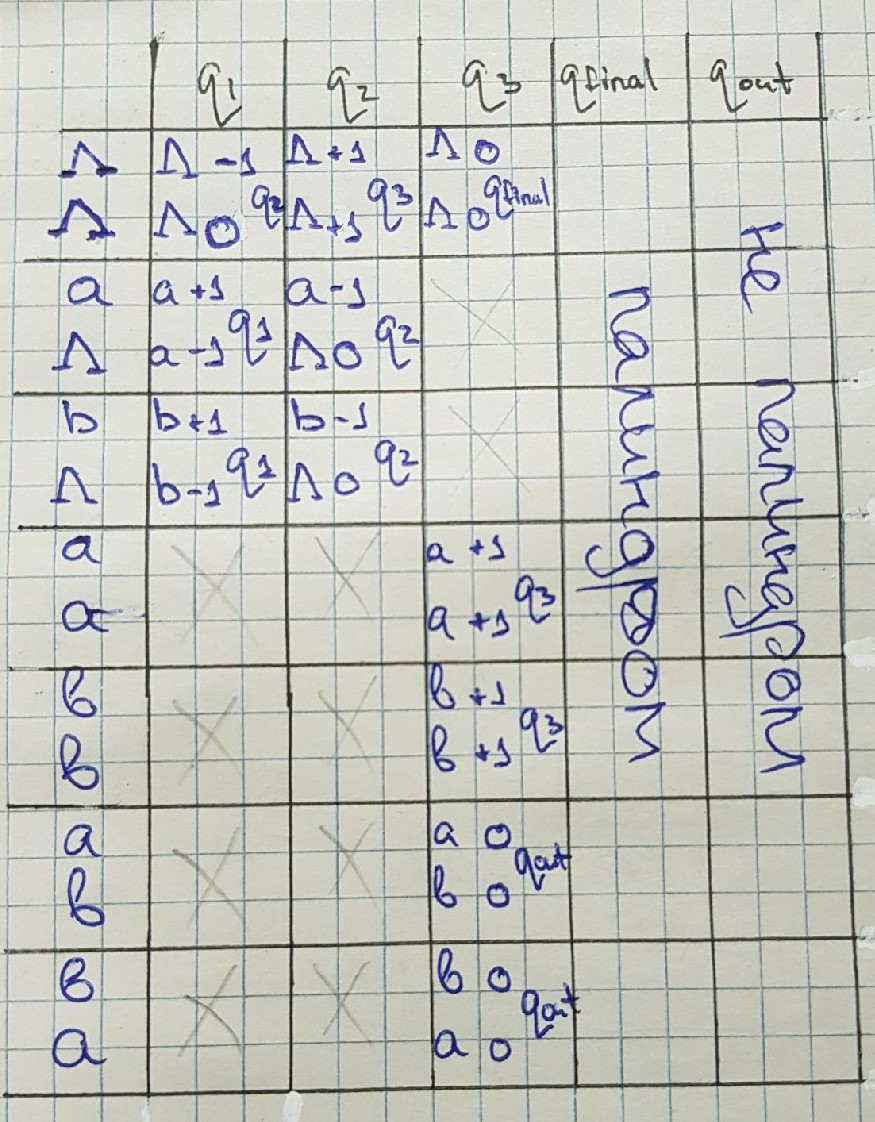
\includegraphics[width=0.7\textwidth]{tabl}

Алгоритм:
\begin{itemize}
\item Сначала, с помощью состояния $q_1$, смещаемся по первой ленте вправо и пишем на вторую ленту те же символы, что и на первой ленте. Когда на первой ленте встретим $\Lambda$, переходим в состояние $q_2$, перемещая головку на первой ленте на первый ненулевой символ (то есть делаем -1).

\item Перемещаем головку на первой ленте в её начало. Когда встречаем $\Lambda$ на первой ленте (что означает, что мы вернулись в её начало) сдвигаем головку верхней и нижней ленты вправо на 1, теперь они обе нахоядся в начале слов на ленте и на второй ленте символы написаны в перевёрнутом порядке по сравнению с первой. (см. работу в состояние $q_2$).

\item С помощью состояния $q_3$ сверяем последовательности символов на первой и на второй лентах (на второй перевёрнутая последовательность). Если находим различие переходим в состояние $q_{out}$, которое говорит, что последовательность не палиндром\\
Если дошли до $\Lambda$, то перевёрнутая последовательность сходится с прямой, значит, слово - палиндром (переходим в конечное состояние $q_{final}$.
\end{itemize}


\section*{Задача 2}
Доказать, что следующие определения перечислимого множества $X \subset {N}$ эквивалентны:
\begin{itemize}
\item Существует алгоритм, печатающий все элементы множества (в любом порядке и со сколь угодно большими паузами между элементами).
\item Множество является областью определения некоторой вычислимой функции.
\item Множество является областью значений некоторой вычислимой функции.
\end{itemize}
$\square$

$(1\Rightarrow3)$
 Можно построить функцию $g(n)$, область значение которой -- $ X $:
Для этого на входе $ n $ запускаюем алгоритм, печатающий элементы -- $ X $, и будем считать количество напечатанных элементов, когда будет напечатан $ n $ый элемент, он будет выдаваться в качестве значения функции $g(n)$ на входе $ n $. Получается, множество значений функции $g$ -- $ X $\\

$(3\Rightarrow2)$
Пусть $X = f(n)$ для некоторой функции f. Опишем алгоритм вычисления функции g, который получает на вход x: перебирает все числа и для каждого числа n вычисляет f(n) и сравнивает с x. 
Если $f(n) = x$, то $g(x) = 1$, иначе - $g(x)$ не определена в х (то есть алгоритм вычисления g не даёт никакого результата), получается, что X - область определения g.\\

$(3 \Rightarrow 1)$
Пусть функция $f(n)$ имеет область значений X. Для каждого натурального числа, если функция f(n) определена, то печатаем результат. Построили алгоритм, печатающий все элементы множества Х и только их.\\

$(2 \Rightarrow 3)$
Пусть $g(x)$ - функция, область значений которой - X. Переопределим g(x) так, что для каждого х из Х $g(x)=x$. Получили, что $Х$ - область значений некоторой вычислимой функции.
\begin{flushright}
	$\blacksquare$
\end{flushright}




\section*{Задача 3}
Задача: найти элемент в массиве длиной n, который встречается более чем $n/2$ раз за 2 прохода по массиву (сложность по времени $\mathcal{O}(n)$) используя память $\mathcal{O}(n\log{}n)$\\

Алгоритм:\\
Создадим 2 переменные:\\
candidat - тут будет лежать элемент, кандитат на нужный нам\\
flag - счётчик\\

Проходимся по массиву циклом и делаем следующие:\\

\begin{itemize}
\item Если переменная flag равна 0, то в переменную candidat кладём текущий элемент, а flag увеличиваем на 1
\item Иначе если текущий элемент равен тому, который в candidat, увеличиваем flag на 1
\item во всех остальных случаях уменьшаем flag на 1
\end{itemize}

После этого прохождения по массиву в переменной condidat будет лежать элемент, который встречается более чем $n/2$ раз, если такой в массиве существует (строго док-ва не привожу, но алгоритм рассказывали в школе, а для интуитивного понимания привели такую ситуацию:\\
n дамм приходят на балл в каких-то разных платьях(например, разного цвета). Если дамма встречает другую с другим платьем, то они садятся. Останутся стоять только даммы в одинаковых платьях.\\
Но в массиве может и не быть нужного элемента, но в переменной candidat все равно что-то будет. Поэтому вторым проходом по массиву проверям существует ли вообще такой элемент.\\
Получаем алгоритм сложность которого $\mathcal{O}(n)$, а требуемая дополнительная память — $\mathcal{O}(1)$ \\
Пример кода алгоритма на python: 

\includegraphics{снимок}

\section*{Задача 4}
Задача: посетить как можно больше мероприятий при условии, что мероприятие можно посещать только полностью, то есть с начала и до конца\\

\begin{itemize}
\item Рассмотрим 1ый жадный алгоритм. Он не является оптимальным, так как существует контрпример:
\begin{center}
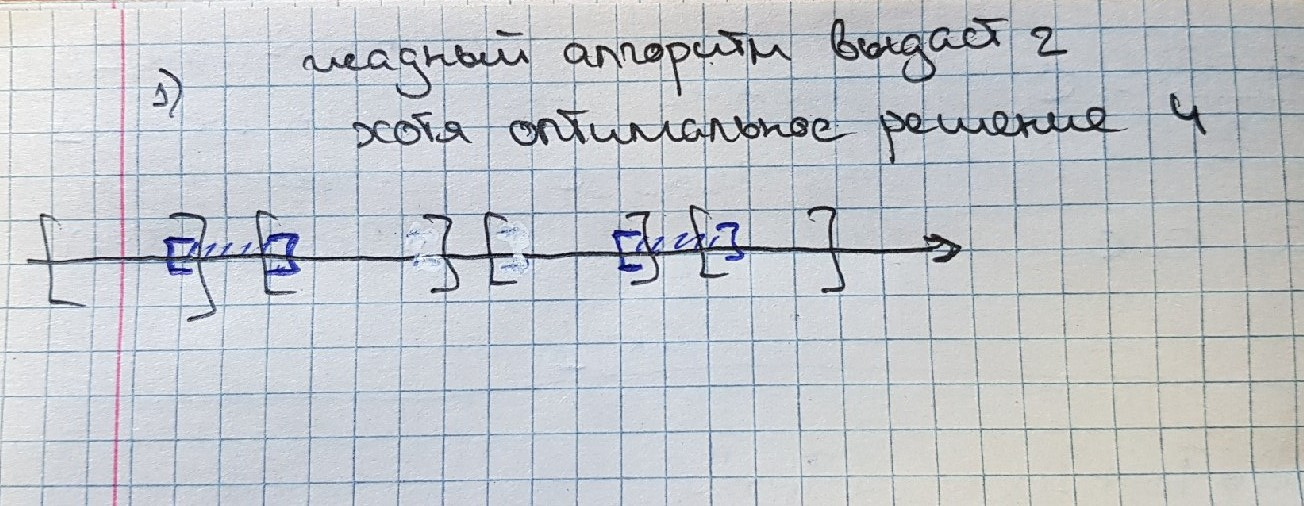
\includegraphics[width=0.7\textwidth]{pic_1}
\end{center}
В нём вместо каждого "короткого: отрезка , который выберет жадный алгоритм, оптимально выбирать 2 других непересекающихся длинных 

\item Рассмотрим 2ой жадный алгоритм. Он не является оптимальным, так как существует контрпример:
\begin{center}
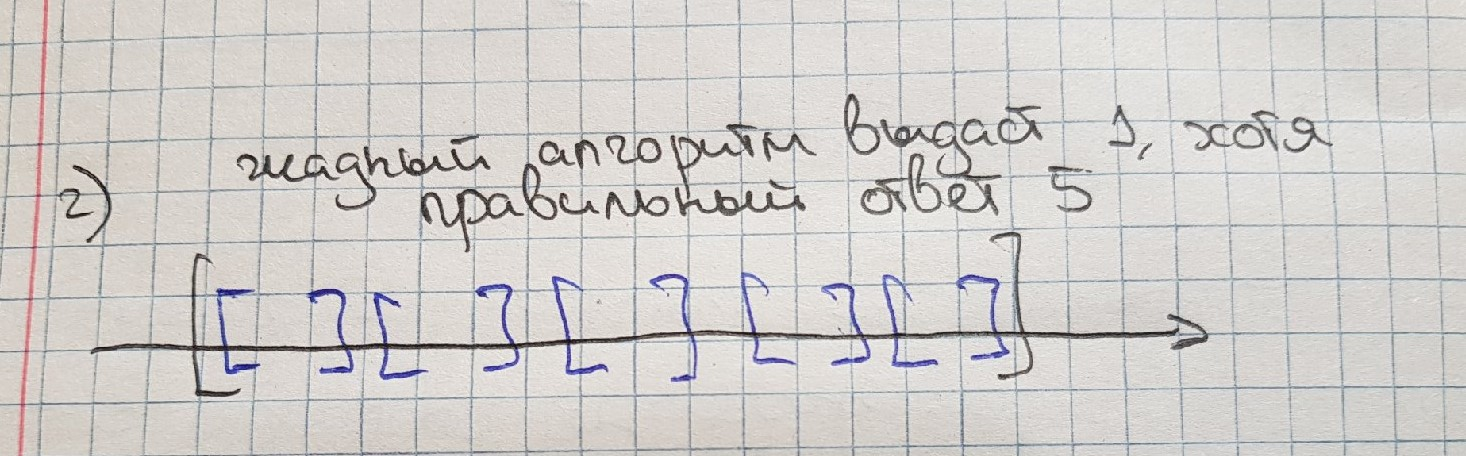
\includegraphics[width=0.7\textwidth]{pic_2}
\end{center}
Вместо одного длинного события, которое начинается раньше всех, оптимально выбирать 5, которые идут последовательно друг за другом во время длинного.

\item 3ий жадный алгоритм является оптимальным, докажем это:\\
От противного. Пусть существует пример, когда наш жадный алгоритм работает не оптимально. Выбирем из таких примеров самый минимальный. Например: \\
жадный алгоритм: $\left[ {1,3} \right)$, $\left[ {4,6} \right)$, $\left[ {6,8} \right)$ \ldots \\
оптимальный алгоритм: $\left[ {2,4} \right)$, $\left[ {4,7} \right)$ \ldots \\
Посмотрим на первую заявку в жадном решении, эта та заявка, которая раньше всех заканчивается, и пусть она не входит в оптимальное решение, значит, первая заявка в оптимальном решении заканчивается позже(не раньше) заявки в жадном решении. Тогда можно поменять первую заявку в жадном решении и оптимальном, то есть в нашем примере поменяем заявки $\left[ {1,3} \right)$ и $\left[ {2,4} \right)$. Теперь в жадном и оптимальном решениях первые заявки одинаковые (если мы так сделаем, ничего не изменится), поэтому мы можем убрать её и перейти к примеру с меньшим количеством заявок. Получаем противоречие с тем, что изначально выбрали минимальный пример. Следовательно этот жажный алгоритм работает всегда оптимально.\\
Сложность алгоритма: $\mathcal{O}(n)$ + $\mathcal{O}(n\log{}n)$\\
Предварительная сортировка по правому пределу ($\mathcal{O}(n\log{}n)$), проход по массиву($\mathcal{O}(n)$) 

\end{itemize}

\section*{Задача 5}
Задача: получить производящую функцию чисел $ BR_{4n+2} $ -- правильные скобочные последовательности длины $ 4n + 2 $\\
Обозначим $ BR_{4n+2} $ за $ T_{2n+1} $. И для чисел Каталана(правильных скобочных последовательностей длины $ n $ известно рекурентное соотношение (дальше будут сложные и не совсем логичные выкладки, берутся они из аналогии для вывода производящей функции для чисел Каталана длины $ 2n $):\\
$ T_{n}=T_{0} T_{n-1}+T_{1} T_{n-2}+\ldots+T_{n-1} T_{0} $, где 
$ T_0 = 1 $\\
Производящая функция в нашем случае (для чисел Каталана, где открывающихся скобок $ 2n+1 $) принимает вид: \\
$ A(x)=T_{1}+T_{3} x+T_{5} x^{2}+\ldots+T_{2 n+1} x^{n}+\ldots $\\
Только нечётные коэффициенты. Рассмотрим также и производящую функцию для чисел Каталана с чётным количеством открывающихся и закрывающихся скобок, то есть с чётными коэффициентами:\\
$ B(x)=T_{0}+T_{2} x+T_{4} x^{2}+\ldots+T_{2 n} x^{n}+\ldots $\\
Возьмём их произведение и преобразуем его:\\
 \[A B=\left(T_{1}+T_{3} x+T_{5} x^{2}+\ldots\right)\left(T_{0}+T_{2} x+T_{4} x^{2}+\ldots\right) \] 
\begin{equation}\label{AB}
 A B=T_{1} T_{0}+\left(T_{3} T_{0}+T_{1} T_{2}\right) x+\left(T_{1} T_{4}+T_{2} T_{3}+T_{5} T_{0}\right) x^{2}+\ldots
\end{equation} 
Из рекурентной формулы заметим, что \\
\[ T_{2}=T_{1} T_{0}+T_{0} T_{1}=>T_{1} T_{0}=T_{2} / 2\]
\[ T_{3} T_{0}+T_{1} T_{2}=T_{4} / 2 \]
\[ T_{1} T_{4}+T_{2} T_{3}+T_{5} T_{0}=T_{6} / 2\] 
И так далее $ \ldots $ Подставляем эти соотношения в формулу \eqref{AB}, получается\\
\begin{equation}\label{AB_new}
 A B=\frac{T_{2}}{2}+\frac{T_{4}}{2} x+\frac{T_{6}}{2} x^{2}+\ldots+\frac{T_{2 n}}{2} x^{n-1+\ldots}
\end{equation} 
Домножаем обе части уравнения \eqref{AB_new} на $ 2x $, в правой части получается $ B(x) $ без первого члена $ T_0 = 1 $, поэтому уравнение \eqref{AB_new} приобретает такой вид:\\
\[ 2 x A B=T_{2} x+T_{4} x+\ldots+T_{2 n} x^{n}+\ldots\]
\begin{equation}\label{num_1}
2 x A B=B-1
\end{equation} 
Нужно получить ещё одно уравнение на производящие функции $ A $ и $ B $, для этого возведём $ B $ и $ A $ в квадрат и снова пользуясь соотношениями из рекурентной формулы для чисел Каталана получим уравнение:\\
\[B^{2}=\left(T_{0}+T_{2} x+T_{4} x^{2}+\ldots\right)\left(T_{0}+T_{2} x+T_{4} x^{2}+\ldots\right) \]
\[B^{2}=T_{0}^{2}+\left(T_{0} T_{2}+T_{2} T_{0}\right) x+\left(T_{0} T_{4}+T_{2} T_{2}+T_{4} T_{0}\right) x^{2}+\ldots \]
Из рекупентной формулы:
\[T_{0}^{2}=T_{1} \]
\[T_{0} T_{2}+T_{2} T_{0}=T_{3}-T_{1}^{2} \]
\[ T_{0} T_{4}+T_{2} T_{2}+T_{4} T_{0}=T_{5}-\left(T_{1} T_{3}+T_{3} T_{1}\right)\]
Получается:
\[ B^{2}=T_{1}+T_{3} x-T_{1}^{2} x+T_{5} x^{2}-\left(T_{1} T_{3}+T_{3} T_{1}\right) x^{2}+\ldots\]
Заметим, то что с минусом в выражении выше немного похоже на $A^2$, распишем $ A^2 $ и получим второе уравнение:
\[A^{2}=\left(T_{1}+T_{3} x+T_{5} x^{2}+\ldots\right)\left(T_{1}+T_{3} x+T_{5} x^{2}+\ldots\right) \]
\[A^{2}=T_{1}^{2}+\left(T_{1} T_{3}+T_{3} T_{1}\right) x+\left(T_{1} T_{5}+T_{3} T_{3}+T_{5} T_{1}\right) x^{2}+\ldots \]
Домножаем $ A^2 $ на $ x $ и получаем выражение:
\begin{equation}\label{num_2}
B^{2}=A-A^{2} x
\end{equation}

Получаем систему из двух уравнений: \eqref{num_1} и \eqref{num_2}, где $ A $ -- производящая функция, которую нужно найти:
\[
\left\{ 
\begin{aligned}
2 x A B=B-1,\\
B^{2}=A-A^{2} x
\end{aligned}
\right.
\]
Из уравнения \eqref{num_1}: $ A=\frac{B-1}{B \cdot 2 x}$ подставляем в уравнение \eqref{num_2}, получаем:
\[ B^{2}=\frac{B-1}{2 x B}-\frac{(B-1)^{2}}{4 B^{2} x^{2}} x\]
\[ 4 x B^{4}=(B-1)(B+1)\]
\[ 4 x B^{4}=B^{2}-1\]
Это квадратное уравнение относительно $ B^2 $, его решения:
\[ B_{12}^{2}=\frac{1 \pm \sqrt{1-16 \cdot x}}{8 x}\]
Выбираем знак из условия, что если в характеристическую функцию поставить $ 0 $, то получится $ T_0 = 1 $, тогда из 
$ 8 x B^{2}=1 \pm \sqrt{1-16 x} $ понятно, что нужно выбирать знак <<->>. В итоге:
\begin{equation}\label{B2}
B^{2}=\frac{1-\sqrt{1-16 x}}{8 x}
\end{equation}
Решаем \eqref{num_2} как квадратное уравнение относительно $ A $, знак корня выбираем из тех же соображений, что и раньше, получаем:
\[ A=\frac{1-\sqrt{1-4 x B^{2}}}{2 x}\]
Подставляем в это выражение значение для $ B^2 $ из \eqref{B2}, получаем ответ для производящей функции $ A $:
\[ A=\frac{1-\sqrt{\frac{1}{2}+\frac{\sqrt{1-16 x}}{2}}}{2 x}\]
Ответ: $ A=\frac{1-\sqrt{\frac{1}{2}+\frac{\sqrt{1-16 x}}{2}}}{2 x} $

\section*{Задача 6}
По условию задачи сразу можно составить рекуренту:
\[ T(n)=3 T\left(\left[\frac{n}{\sqrt{3}}\right]-5\right)+\theta\left(10 \frac{n^{3}}{\log n}\right)\]
Заметим, что при больших $ n $ константа $ -5 $ очень мала по сравнению с тем, что мы делим на $ \sqrt{3} $, следовательно ей и целым округлением можно пренебречь, получим:
\[ T(n)=3 T\left(\frac{n}{\sqrt{3}}\right)+\theta\left(\frac{n^{3}}{\log n}\right)\]
Распишем, как меняется сумма уровня дерева от глубины и найдём закономерность
\[ \frac{n^{3}}{\log n} \rightarrow 3 \cdot \frac{\frac{n^{3}}{(\sqrt{3})^{3}}}{\log \left(\frac{n}{\sqrt{3}}\right)}=\frac{\frac{n^{3}}{\sqrt{3}}}{\log \left(\frac{n}{\sqrt{3}}\right)}\rightarrow 9 \cdot \frac{\frac{n^{3}}{(\sqrt{3})^{3}}}{\log \left(\frac{n}{(\sqrt{3})^{2}}\right)}=\frac{\frac{n^{3}}{\sqrt{3}}}{\log \left(\frac{n}{(\sqrt{3})^{2}}\right)}\]
И так далее, в итоге можем записать $ k $ый элемент:
$ \frac{\frac{n^{3}}{(\sqrt{3})^{k}}}{\log \left(\frac{n}{(\sqrt{3})^{k}}\right)}$\\
Глубина рекурсии будет равна $ \log n $, так как каждый раз мы делим на $ \sqrt{3} $, поэтому кол-во операций, которое сделает наш алгоритм эта следующая сумма:
\[T(n)=\sum\limits_{k=0}^{\log (n)} \frac{\frac{n^{3}}{(\sqrt{3})^{k}}}{\log \left(\frac{n}{(\sqrt{3})^{k}}\right)} \]
Снизу эту сумму можно оценить первым членом при $ k = 0 $ (понятно, что вся сумма больше первого члена суммы, так как все числа положительные), то есть  
\begin{equation}\label{niz}
T(n) = \Omega(\frac{n^{3}}{\log n})
\end{equation}
Пусть сверху сумма также оценивается первым членом, докажем это по индукции по глубине рекурсии, то есть 
$\exists C > 0, \forall k < \log(n) \longrightarrow T(k) < C\frac{k^{3}}{\log k}  $\\ 
База индукции: $k = 0$, тогда сумма представляет собой первое слагаемое и равна $\frac{n^{3}}{\log n}$. Доказано\\
Шаг индукции: Пусть доказано для $k < m$, докажем для $k = m$: \\
По предположению индукции верно:
\[\exists C>0: \exists N>0: \forall n \geq N \mapsto \sum_{k=0}^{m-1} \frac{\frac{n^{3}}{(\sqrt{3})^{k}}}{\log \left(\frac{n}{(\sqrt{3})^k}\right)} \leq C \frac{n^{3}}{\log n}\]
Преобразуем слагаемое с номером m и оценим его:
\[ \frac{\frac{1}{(\sqrt{3})^{m}}}{\log \left(\frac{n}{(\sqrt{3})^m}\right)} = \frac{1}{(\sqrt{3})^{m}(\log n-m \cdot \log (\sqrt{3}))}
\]\\
\[
\frac{1}{(\sqrt{3})^{m}(\log n-m \cdot \log (\sqrt{3}))} \leq C \frac{1}{\log n}
\]
\[
\log n \leq C(\sqrt{3})^{m}(\log n-m \log \sqrt{3})
\]
\[
m \log \sqrt{3} \leq\left(C \cdot(\sqrt{3})^{m}-1\right) \log n
\]
\[
m \leq \frac{\left(C(\sqrt{3})^{m}-1\right)}{\log \sqrt{3}} \log n
\]
Всегда найдутся С и N такие, что неравенство выполняется, для $\forall m < \log(n) $. Тогда слагаемое с номером m можно оценить сверху $C \frac{1}{\log n}$.
Сложим это неравенство с неравенством из предположения индукции: для  $С_2 > C_1 + C$ и $N_2 = max(N_1, N)$ выполняется:
\[\exists C_2>0: \exists N_2>0: \forall n \geq N_2 \mapsto \sum_{k=0}^{m} \frac{\frac{n^{3}}{(\sqrt{3})^{k}}}{\log \left(\frac{n}{(\sqrt{3})^k}\right)} \leq C_2 \frac{n^{3}}{\log n}\]
Следовательно, шаг индукции доказан.

Таким образом, $O(\frac{n^3}{\log n})$ оценка сверху, следовательно\\ 
Ответ: $T(n) = \Theta\left(\frac{n^3}{\log n}\right)$


\end{document} % конец документа
